
\subsection{Part-of-speech tagging}

This section will go into the details of the Part-of-speech task, what the
specifics are, considerations in regards to the data used, any issues we came
across, and the results of our experiments.

\subsubsection{Task definition}

The Part-of-Speech task is a classification task where the objective is to label
each word in a sentence with it's corresponding part-of-speech label such as
noun, verb, adjective, etc. Eg. the sentence ``Our work is done'' would be
labeled ``determiner noun auxiliary verb''.

For our dataset, there are around 17 different labels, but some languages don't
use all of them. The same words can have different labels in different context,
so the classifier should be able to figure out which label is a better fit on a
sentence by sentence basis. Simply remembering that word $X$ has label $Y$
wouldn't be able to generalize very well.

The performance of a classifier for the POS task is the simple accuracy of the
predictions. Since there is no label which is a lot more common than others,
guessing randomly would result in a very poor score. 

\subsubsection{Data}

For this task we used datasets from~\ref{}{UniversalDependencies.org} which has
a broad selection of languages with multiple datasets (called treebanks) in
each. The datasets are all in the CoNNL-U format, but are created from different
types of sources. The source types are given as tags such as news, legal, blog,
wiki, etc. As it is unclear how much of the data is made from each of the
sources given, we prefered datasets made from single source types to keep the
datasets similar to the best of our abilities.

Since the datasets are already split, these were concatenated before splitting
into our own sizes. Concatenation happened using the command ``cat *.conllu >
combined.conllu'', since the convention for the datasets is to name the files
something with train, test, and dev, the assumed order of the files is dev,
test, and train. Meaning that if the dev set (eg.\ the validation set) contains
5000 sentence, only these were used in our datasets, and none of the sentences
from the test or training sets would be used. No guarantees however were made to
guarantee this ordering, so depending on the naming conventions used in the
specific treebanks this may differ. This shouldn't matter however since there
shouldn't be any difference between the data in the different files.

Some datasets, such as the Norwegian dataset, contains contractions alongside
the individual words. Since the contration is usually unlabelled in the datasets
these were simply removed from the data for ease of parsing. This has the
obvious consequence that the models are not trained on the contractions of words
which are often more commonly used, this however shouldn't affect the
comparisons between word orderings since contractions shouldn't affect these and
the test data would also be using the same convention where contractions are
split. An alternative approach would be to create two sentences, one using the
contraction and another without. This would be a way to extend the dataset and
learn to properbly tag both the individual words and their contraction.

The treebanks we selected were all made from news, where some used additional
sources such as non-fiction and spoken. A list of the languages, their
respective treebank selected, and their tags is given below.

* Arabic,   PADT, news

* Hindi,    HDTB, news

* Urdu,     UDTB, news

* Japanese, GSD, blog, news

* Danish,   DDT, fiction, news, non-fiction, spoken

* Norwegian,Bokmaal, blog, news, non-fiction

* Russian,  SynTagRus, fiction, news, non-fiction

The distribution of tokens, labels, etc. is given in figure \ref{}.

\subsubsection{Results and analysis}

Looking at the results of the experiments, we mainly focus on the case where the
models trained with early stopping and a maximum of 50 epochs. As such, we where
interested in seeing how the models converged with different batch sizes aswell
as with and without the CRF layer. The average number of epochs run for each
framework implementation is shown in Table~\ref{table:epochs-run-pos}.

\begin{table}[h!]
    \centering
    \begin{tabular}{l c c c|c c c}
        \toprule
        \multirow{2}{*}{\bfseries Batch size}     &
        \multicolumn{3}{c}{\bfseries Bi-LSTM}     &
        \multicolumn{3}{c}{\bfseries Bi-LSTM-CRF} \\
        \cmidrule(lr){2-7}
        & DyNet & PyTorch & TensorFlow
        & DyNet & PyTorch & TensorFlow \\
        \cmidrule(lr){1-7}
         1 & 13.60 & 21.44 & 36.43 & 13.26 &  8.09 &  5.23 \\
         8 & 17.31 & 39.86 & 49.71 & 16.55 & 16.20 &  7.91 \\
        32 & 22.57 & 48.83 & 50.00 & 23.78 & 22.40 & 10.66 \\
        \bottomrule
    \end{tabular}
    \caption{Average of epochs run across all seeds and languages when trained
        with early stopping.
    }\label{table:epochs-run-pos}
\end{table}

From the data it is clear, that an increase in batch size also means that the
model takes longer to converge. This is expected, as the number of
backpropagation operations decrease when the input data is split into larger
mini-batches (eg.\ when working with 4000 sentences and a batch size of 1, each
epoch will update its weights 4000 times. This number drops to
$\frac{4000}{32}=125$ when the batch size is 32).

We also see, that adding a CRF layer dramatically decrease the time it takes for
the models to converge. With the standard \texttt{Bi-LSTM} model implemented in
TensorFlow, none of our experiments reached a point of convergence within the
upper bound on the number epochs, and for PyTorch with batch size 32 and
TensorFlow with batch size 8 the average number also indicate that only very few
training sessions reached the point of convergence before the epoch limit. This
also suggests, that we set the upper bound to strict.

It is a completely different story for the \texttt{Bi-LSTM-CRF} models. Here,
all experiments terminated early and the relation between the frameworks
changed.  DyNet had an almost identical epoch average, but PyTorch saw a more
than 50\% drop and for TensorFlow the drop was more than 80\%. The explanation
for this could be, that the 2 layer \texttt{Bi-LSTM} of the DyNet implementation
is a more efficient model than the regular \texttt{Bi-LSTM} with only 1 layer,
and that the addition of a CRF layer is insignificant (in terms of the time it
takes to find a convergence point). For the PyTorch and TensorFlow
implementation, however, it seems that the CRF layer greatly helps the
sequential model to converge.

We do find it odd, though, that the TensorFlow implementation on average across
batch sizes takes less than 10 epochs to find a satisfying convergence point.

When we turn our attention to the accuracy achieved by the models, we see the
results reflect the epoch numbers. In
Figure~\ref{chart:acc-by-batch-and-lang-pos} the results are plotted
according to batch size and language. A table of all the data can be found in
Table~\ref{table:acc-total-pos}.

\begin{figure}[h!]
    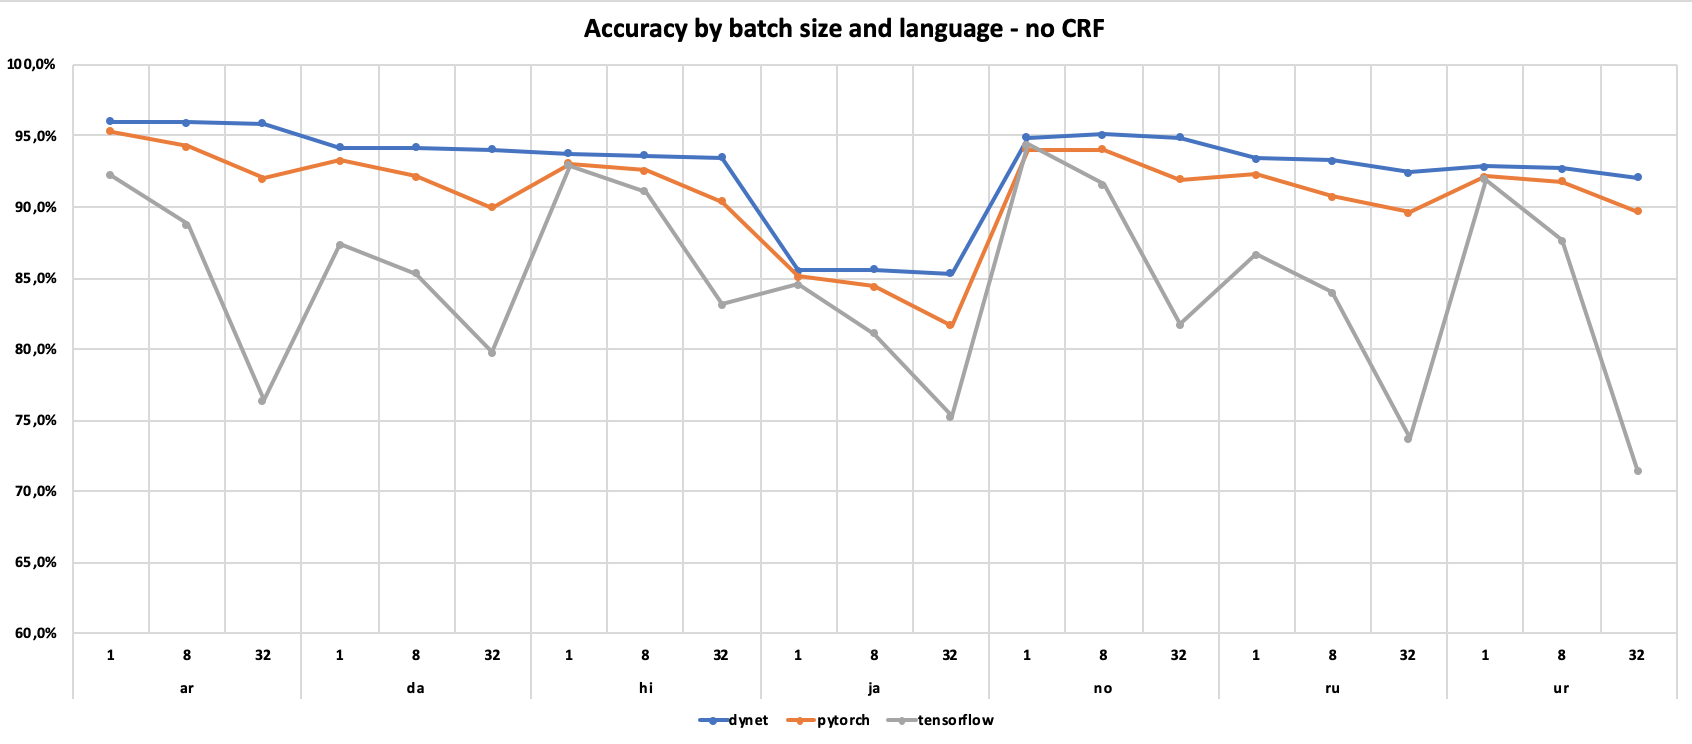
\includegraphics[width=\textwidth]{accuracy-pos-no-crf}
    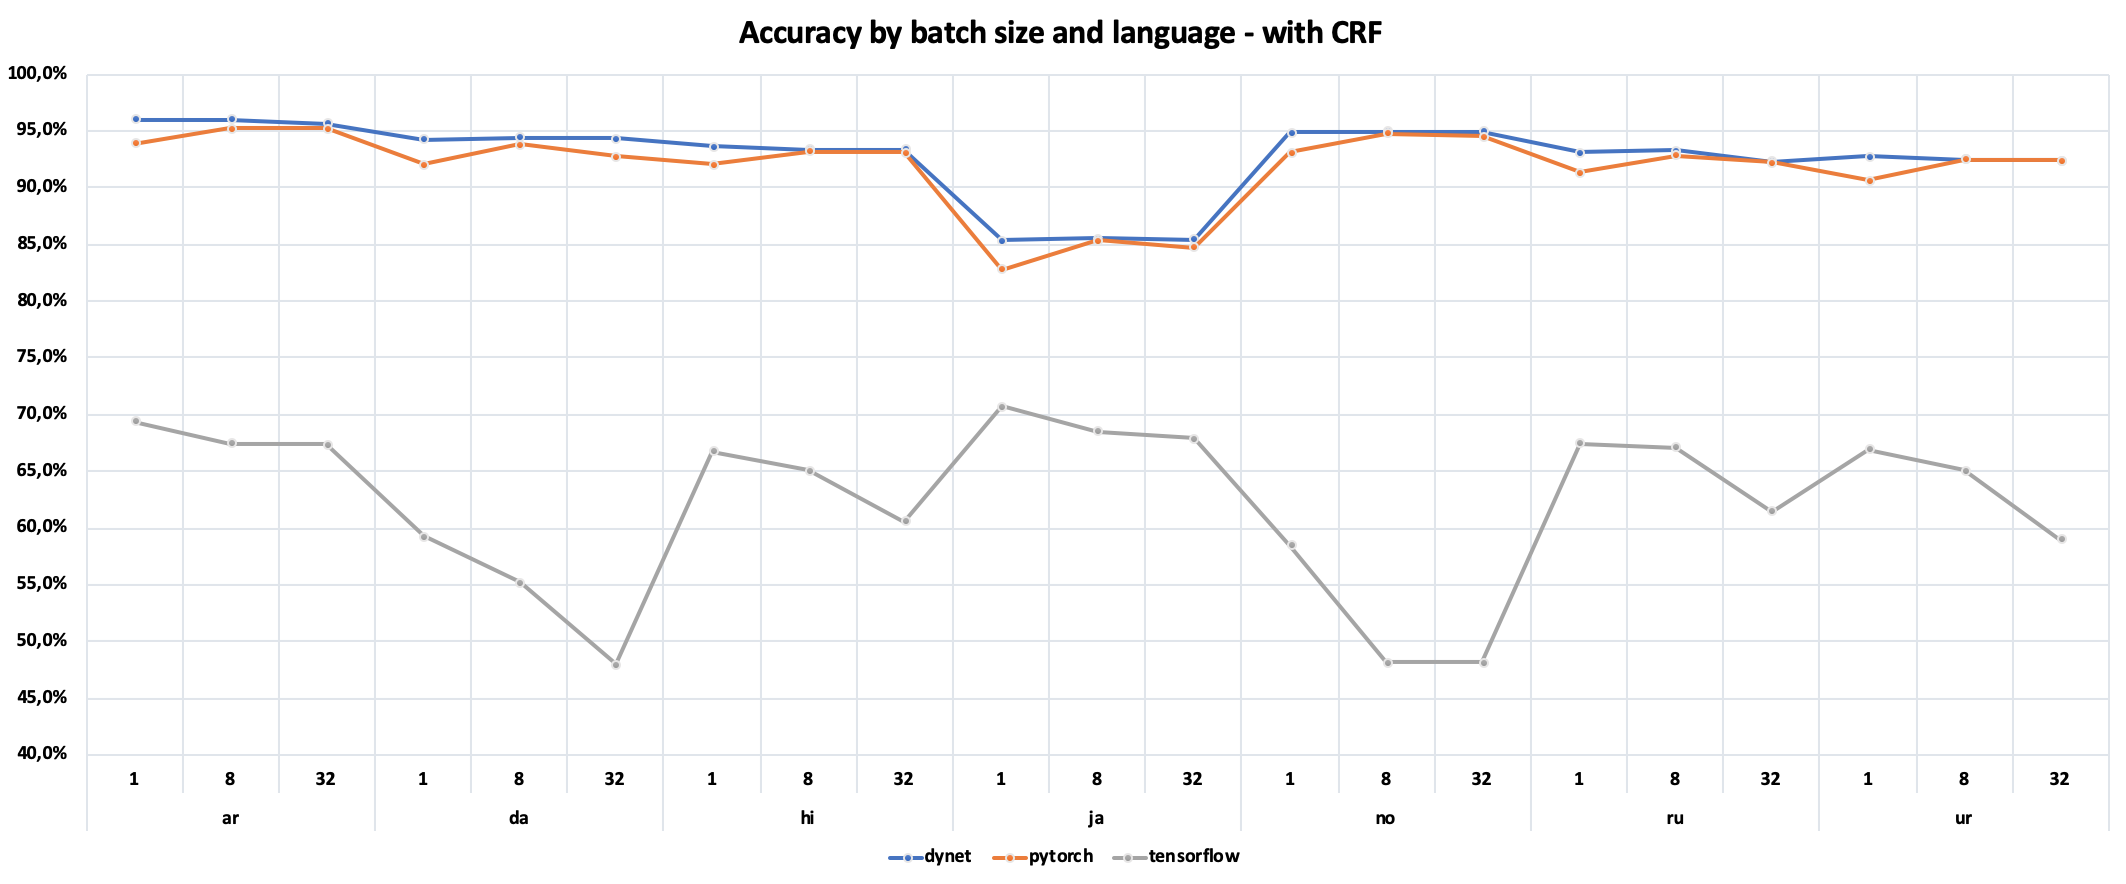
\includegraphics[width=\textwidth]{accuracy-pos-with-crf}
    \caption{Average accuracy across seeds with early stopping and a maximum of
        50 epochs. The x-axis is batch size 1, 8 and 32 for all languages in the
        experiments. Top: Results for \texttt{Bi-LSTM}. Bottom: Results for
    \texttt{Bi-LSTM-CRF}. \textbf{NB:} Notice different y-axises.
    }\label{chart:acc-by-batch-and-lang-pos}
\end{figure}

The results show that the non-CRF models perform quite simiar for most languages
when the batch size is 1 (except for the TensorFlow implementation, which
underperforms severely for arabic, danish and russian). This is in compliance
with the fact, that all models terminated training before reaching the maximum
number of epochs and as such found a state where the accuracy on the validation
set stopped increasing. The similarities in performance is a good measurement
that these models found a somewhat optimal tuning of their respective weights.

This seems even more obvious when looking at the results for the
\texttt{Bi-LSTM-CRF} models. Here, the DyNet and the PyTorch implementation are
near identical, with a small advantage for DyNet in most cases. Furthermore,
larger batch sizes mostly seem to erradicate the small difference in performance
between the two, which also corresponds to what we would expect from the models
since both the PyTorch and the DyNet implementation converged within less than
25 epochs.

In the cases where the models did not get to properly converge (ie.\ the
implementation of \texttt{Bi-LSTM} in TensorFlow with batch size 8 and 32 and in
PyTorch with batch size 32), the accuracy achieved is also considerably worse
than the DyNet implementation, which terminated training before 25 epochs for
all batch sizes. Its also worth noticing, that the PyTorch implementation with
batch size 8 is also doing notably worse even though it did seem to converge,
albeit at a higher epoch number of 39.86. Since TensorFlow with a batch size of
1 is also doing worse on average and spent more than 30 epochs converging, we
may see that the eventual convergence after 30 epochs is in risk of ending up in
a sub-optimal state (ie.\ gets stuck in a local minima that is not optimal).

The outlier here is the TensorFlow implementation. 

\begin{table}[h!]
    \centering
    \begin{tabular}{c l c c c|c c c}
        \toprule
        \multirow{2}{*}{\bfseries Language} &
        \multirow{2}{*}{\bfseries Batch size} &
        \multicolumn{3}{c}{\bfseries Bi-LSTM} &
        \multicolumn{3}{c}{\bfseries Bi-LSTM-CRF} \\
        \cmidrule(lr){3-8}
        && DyNet & PyTorch & Tensorflow & DyNet & PyTorch & Tensorflow \\

        \cmidrule(lr){1-8}
        \multirow{3}{*}{\bfseries ar}
        &  1 & 96.0\% & 95.3\% & 92.2\% & 96.0\% & 93.9\% & 69.4\% \\
        &  8 & 96.0\% & 94.3\% & 88.8\% & 96.0\% & 95.2\% & 67.5\% \\
        & 32 & 95.8\% & 92.0\% & 76.4\% & 95.8\% & 95.3\% & 67.4\% \\

        \cmidrule(lr){1-8}
        \multirow{3}{*}{\bfseries da}
        &  1 & 94.2\% & 93.2\% & 87.4\% & 94.3\% & 92.1\% & 59.3\% \\
        &  8 & 94.2\% & 92.2\% & 85.4\% & 94.4\% & 93.8\% & 55.2\% \\
        & 32 & 94.1\% & 90.0\% & 79.8\% & 94.3\% & 92.8\% & 47.9\% \\

        \cmidrule(lr){1-8}
        \multirow{3}{*}{\bfseries hi}
        &  1 & 93.8\% & 93.0\% & 92.9\% & 93.6\% & 92.0\% & 66.8\% \\
        &  8 & 93.7\% & 92.6\% & 91.1\% & 93.4\% & 93.2\% & 65.0\% \\
        & 32 & 93.5\% & 90.4\% & 83.1\% & 93.4\% & 93.1\% & 60.6\% \\

        \cmidrule(lr){1-8}
        \multirow{3}{*}{\bfseries ja}
        &  1 & 85.5\% & 85.1\% & 84.6\% & 85.4\% & 82.8\% & 70.8\% \\
        &  8 & 85.6\% & 84.4\% & 81.1\% & 85.5\% & 85.3\% & 68.5\% \\
        & 32 & 85.3\% & 81.7\% & 75.3\% & 85.3\% & 84.7\% & 67.9\% \\

        \cmidrule(lr){1-8}
        \multirow{3}{*}{\bfseries no}
        &  1 & 94.9\% & 94.0\% & 94.4\% & 94.9\% & 93.1\% & 58.5\% \\
        &  8 & 95.1\% & 94.0\% & 91.6\% & 95.0\% & 94.8\% & 48.1\% \\
        & 32 & 94.9\% & 91.9\% & 81.8\% & 94.9\% & 94.5\% & 48.1\% \\

        \cmidrule(lr){1-8}
        \multirow{3}{*}{\bfseries ru}
        &  1 & 93.4\% & 92.3\% & 86.7\% & 93.1\% & 91.3\% & 67.5\% \\
        &  8 & 93.3\% & 90.7\% & 84.0\% & 93.3\% & 92.8\% & 67.1\% \\
        & 32 & 92.4\% & 89.6\% & 73.7\% & 92.3\% & 92.3\% & 61.5\% \\

        \cmidrule(lr){1-8}
        \multirow{3}{*}{\bfseries ur}
        &  1 & 92.9\% & 92.1\% & 91.9\% & 92.7\% & 90.6\% & 67.0\% \\
        &  8 & 92.7\% & 91.8\% & 87.6\% & 92.5\% & 92.5\% & 65.0\% \\
        & 32 & 92.1\% & 89.7\% & 71.4\% & 92.2\% & 92.4\% & 59.0\% \\
        \bottomrule
    \end{tabular}
    \caption{Table with a lot of exciting data.
    }\label{table:acc-total-pos}
\end{table}




\pagebreak
